\section{Tracking und Stabilisierung der Kugelpositionen}\label{kap:tracking}
Wie in Kapitel \ref{kap:detektion} beschrieben, wurde eine Live-Detektion implementiert, welche kontinuierlich
die Bilder der Kamera ausliest, eine Detektion ausführt und anschliessend die Positionen der Kugeln über den Projektor
visualisiert.
Aufgrund von Rauschen auf den Eingabebildern wird die Position jeder Kugel nicht immer an der exakt gleichen Stelle wie
in der vorherigen Detektion erkannt. Dadurch entsteht auf dem Tisch ein unerwünschtes Rauschen in der Position der Kugeln,
was sich durch schnelle, kleine Bewegungen der dargestellten Kreise bemerkbar macht.
Dieses Problem ist in Abbildung \ref{fig:tracking_detected_positions_over_time} visualisiert.
Diese Unruhige Darstellung gilt es zu verbessern, damit der Spieler während des Stosses nicht davon abgelenkt wird.

\begin{figure}[h!]
    \begin{center}
        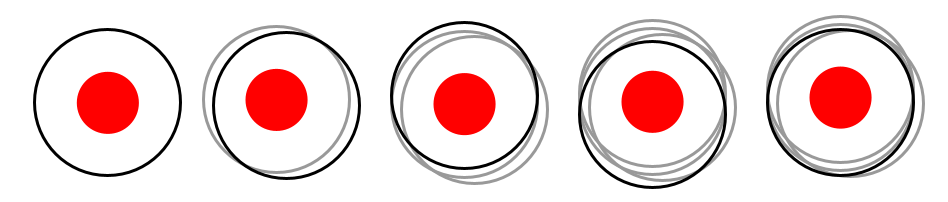
\includegraphics[width=0.6\linewidth]{../common/03_billiard_ai/resources/tracking_detected_positions_over_time.png}
    \end{center}
    \caption{Visualisierung des Rauschens in den detektierten Positionen einer roten Kugel über fünf Frames. Die schwarzen Kreise visualisieren die im entsprechenden Frame detektierte Position, die grauen Kreise die zuvor detektierten Positionen.}
    \label{fig:tracking_detected_positions_over_time}
\end{figure}

Der Lösungsansatz ist die Betrachtung des Spielstandes über die Zeit, um die detektierten Positionen abzuglätten und
das Rauschen zu unterdrücken.
Dies erfordert ein Tracking, welches die detektierten Kugeln von einem Frame $F_{t-1}$ mit den detektierten Kugeln
von Frame $F_{t}$ verbindet. Es muss demnach bestimmt werden, wo eine Kugel aus Frame $F_{t-1}$ in Frame $F_{t}$ ist.

Um dies zu erreichen, wird jede Kugel $K_{t}$ im aktuellen Frame $F_{t}$ geprüft und diejenige Kugel $K_{t-1}$
in Frame $F_{t-1}$ gesucht, die der Kugel $K_{t}$ in der euklidischen Distanz am nächsten ist.
Das bedeutet, es wird zu jeder aktuellen Kugel die Vorgängerkugel aus dem vorherigen Frame gesucht.

Für diese Zuweisung sind bewegte Kugeln problematisch.
Im Fall, dass sich Kugel $K_{t}$ weit von ihrer Position in Frame $F_{t-1}$ entfernt hat,
könnte es zu einer Verwechslung kommen, weil die richtige Kugel nicht mehr die Nächstgelegene ist.
Daher darf die Distanz der nächsten Kugel aus Frame $F_{t-1}$ eine Maximaldistanz $D$ nicht überschreiten.
Diese Maximaldistanz $D$ muss kleiner als der Radius der Kugeln gewählt werden, damit möglichst keine Verwechslungen
auftreten. Ausserdem muss diese Maximaldistanz grösser als das durchschnittliche Rauschen in der detektierten Position
sein, damit das Tracking bei stillstehenden Kugeln erfolgen kann.

Diese Suche nach der nächstgelegenen Kugel des vorherigen Frames wird für jede Kugel des aktuellen Frames durchgeführt.
Kugeln des vorherigen Frames, welche einer aktuellen Kugel zugewiesen wurden, werden nicht erneut zugewiesen.
Kugeln, für die keine Vorgängerkugel gefunden werden konnte, werden als \emph{nicht getrackt} markiert.

Für jede getrackte Kugel können die detektierten Positionen über ein Zeitfenster von $N$ Frames aufgezeichnet werden.
Diese History der Positionen kann anschliessend genutzt werden, um einen \emph{gleitenden Durchschnitt} \cite{wiki:moving_average}
der Position zu berechnen.
Der gleitende Durchschnitt führt bei stillstehenden Kugeln zu einer deutlichen Reduktion des Rauschens.
Bei bewegten Kugeln ist zu beachten, dass diese nicht zwingend über alle Frames getrackt werden können,
weil sie zwischen den Frames zu weit gerollt sein könnten.
Die History wird für Kugeln, die nicht mehr getrackt werden konnten, geleert.
Sobald eine Kugel wieder erfolgreich getrackt werden konnte, wird die History erneut befüllt.
Die Berechnung des gleitenden Durchschnitts auf einigen wenigen Positionen aus der History ist suboptimal, weil
zu wenige Datensätze vorhanden sind, um eine effektive Rauschunterdrückung zu erreichen.
Um dieses Problem zu lösen, wird die Durchschnittsposition einer getrackten Kugel erst verwendet,
wenn diese mindestens $L$ Frames getrackt wurde, wobei $L < N$.
Sofern eine Kugel beispielsweise erst 3 Frames lang getrackt wurde, wird noch kein gleitender Durchschnitt berechnet.
Bei stillstehenden Kugeln ist diese Bedingung unproblematisch, weil diese bei kleinem $L$ schnell erfüllt ist.

Bei bewegten Kugeln ist die Durchschnittsposition weiterhin problematisch, weil diese zwischen den detektierten Positionen liegt und
dadurch hinter der tatsächlichen Position zurückliegt, siehe Abbildung \ref{fig:tracking_moving_average_for_moving_balls}.

\begin{figure}[h!]
    \begin{center}
        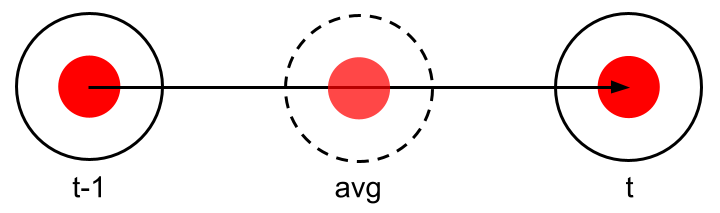
\includegraphics[width=0.6\linewidth]{../common/03_billiard_ai/resources/tracking_moving_average_for_moving_balls.png}
    \end{center}
    \caption{Detektierte Positionen derselben Kugel zum Zeitpunkt $t-1$ und $t$. Der Durchschnitt dieser beiden Positionen liegt hinter der aktuellen Position.}
    \label{fig:tracking_moving_average_for_moving_balls}
\end{figure}

Diese Problematik wird entschärft, indem die Durchschnittsposition $P_{avg}$ mit der aktuellen Position $P_{current}$
aufgrund ihrer Distanz $d$ zusammengerechnet wird \cite{learnopencv:stabilizing_landmarks_in_videos}.
Sofern die Distanz der beiden Positionen gross ist, soll die aktuelle Position verwendet werden, weil in diesem Fall
die Durchschnittsposition zeitlich verzögert hinter der Position liegt, siehe Abbildung \ref{fig:tracking_moving_average_for_moving_balls}.
Sofern die Distanz klein ist, dann kann die Durchschnittsposition verwendet werden, um das Rauschen zu unterdrücken.
Der Faktor $f \in [0; 1]$, mit dem die beiden Positionen kombiniert werden, wird über die Maximaldistanz $D$ des Trackings wie folgt definiert:
\begin{align}
    f = min(\frac{d}{D}, 1)
\end{align}

Das Minimum verhindert, dass $f > 1$ wird, wenn die Distanz $d > D$.
Anschliessend kann der Faktor $f$ verwendet werden, um die geglättete Position $P_{new}$ einer getrackten Kugel zu berechnen:
\begin{align}
    P_{new} = f \cdot P_{current} + (1 - f) \cdot P_{avg}
\end{align}

Für Kugeln, welche nicht getrackt werden konnten, wird die im aktuellen Frame detektierte Position verwendet.

Das Tracking von bewegten Kugeln bedingt, dass sich die Kugeln zwischen zwei aufeinanderfolgenden Frames nicht zu weit
bewegen, um noch immer als dieselbe Kugel identifiziert zu werden.
Dies ist bei kleinen Geschwindigkeiten unproblematisch, allerdings treten bei höheren Geschwindigkeiten
\emph{motion blur} auf und die Kugeln \emph{teleportieren} von einem Ort zum anderen.

Damit ist eine Rauschunterdrückung in der Anzeige der detektierten Positionen aller Kugeln erreicht, ohne dabei eine
sichtbare Latenz zu verursachen.
Es gilt zu beachten, dass das hier vorgestellte Tracking lediglich zum Zweck hat, die dargestellten Positionen zu stabilisieren
und nicht schnell bewegende Kugeln über mehrere Frames tracken zu können.

